\chapter{Work Completed}\label{C:work}
\section{Substrate Mounting}
The proposal initially outlined the design of a mount/fastener for the substrate stack, to integrate a heat spreader, and to better ensure centering and thermocouple placement. Initial meetings with the on-site workshop and design started early with rough sketch designs and discussions on material and manufacture. However, it was quickly decided that focus should be shifted elsewhere in the project and this be returned to at a later date if needed, as the substrate is a shared component of the two projects centred around this experimental setup, and the development new droplet dispensing was the true focus of this project.

\section{Pipette and Mechanical Mounting}
Given the decision for the new rig to be centred around an electronic pipette, as opposed to the manual syringe, a new mounting assembly was needed to secure the pipette to the XYZ stage, ensure there is minimal play and backlash, and position its tip above the substrate for droplet dispensing.

\begin{figure}
    \centering
    \begin{subfigure}{.3\textwidth}
      \centering
      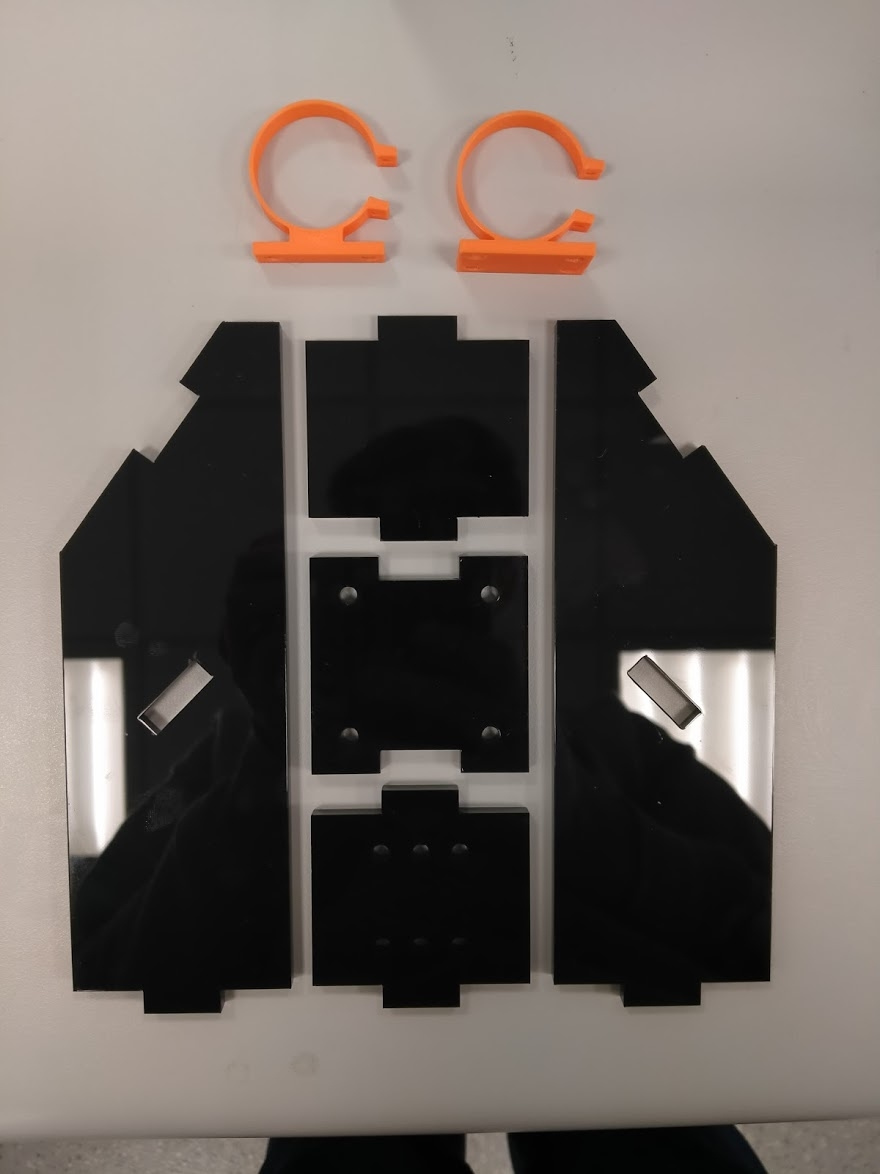
\includegraphics[height=\linewidth]{img/Tower_pcs.jpg}
      \caption{Unassembled Tower}
    \end{subfigure}%
    \begin{subfigure}{.3\textwidth}
      \centering
      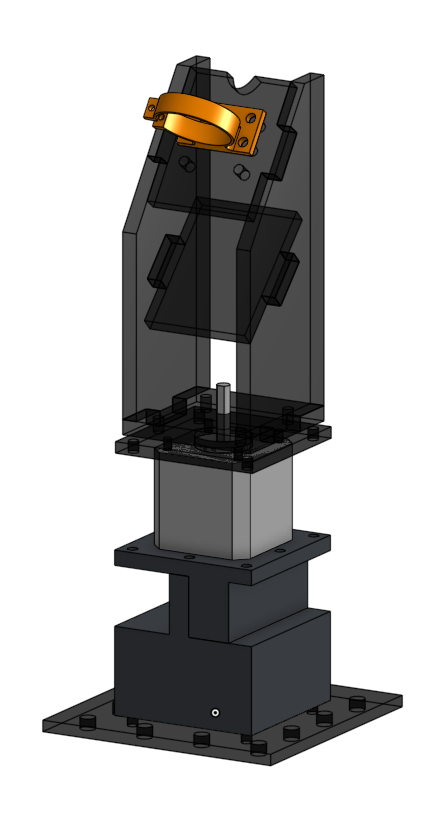
\includegraphics[height=\linewidth]{img/motor_cad_mouting.png}
      \caption{CAD Design}
    \end{subfigure}
    \begin{subfigure}{.3\textwidth}
        \centering
        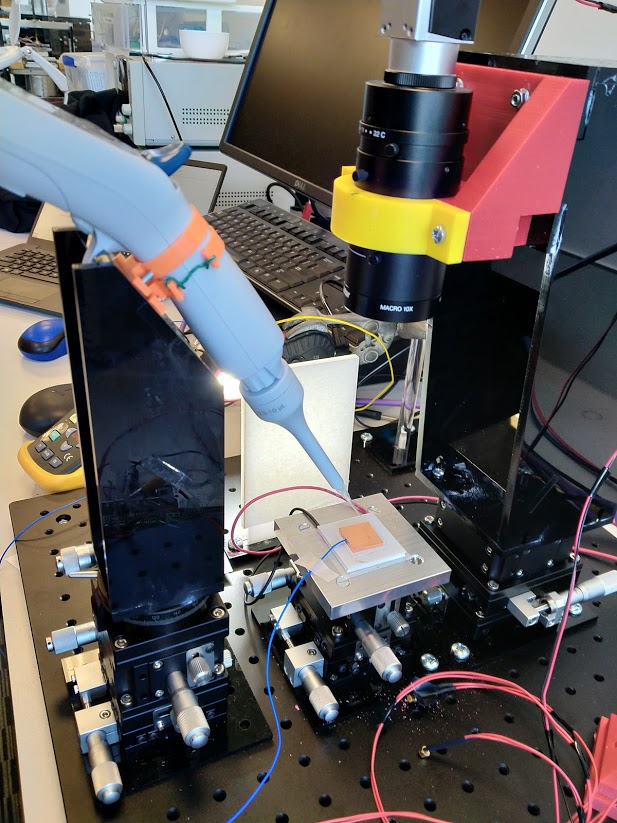
\includegraphics[height=\linewidth]{img/Tower_ass.jpg}
        \caption{Tower Assembled}
      \end{subfigure}
    \caption{Pipette Tower}
    \label{fig:tower}
  \end{figure}

\textbf{Requirements:} The pipette had to be held at 150mm from the top of the optical stage, at 36 degrees. Finer adjustments to be made with the XYZ micrometre controls. 

A tower [\ref{fig:tower}] was designed as the mounting solution. It was constructed from laser cut 6mm acrylic as it had been successfully used in other parts of the existing rig, could be very quickly manufactured to allow rapid prototyping, and producing of a variety of mounting points and different plates. Assembly was left open to allow for access and modification. A taller than final tower design was cut to allow for the new procedure to be carried out before the motorised system was complete.  

\subsection{Interactions and Difficulties}
The electronic pipette formfactor is very 'organic', so the clamping mechanism to fit it to the tower plate itself was challenging to design to successfully restrict its rotation and backlash.  
The base design used to accomplish this was a 3D-printed ring clamp [see \ref{fig:tower}:a] meant to be tightened and fit to the unique form of the pipette body. A variety of ring sizes and gap distance were printed and test fitted. From this I determined that a ring diameter of 32mm and a gap of 6mm fits and deforms to the shape of the pipette. However, there was still some rotation and slip so a notch was cut into the acrylic to slot the pipettes support rest and a second ring clamp attached lower down of the body. 

\section{Electronic Design and Part Selection}

The electronic design for this project is as follows:
A microcontroller provides control signals to step/direction drivers for two stepper motors. One stepper motor controls the tower rotation and the other the optical stage z-axis. The controller also interfaces with the electronic pipette to trigger a droplet release.

\begin{figure}[h]
    \centering
    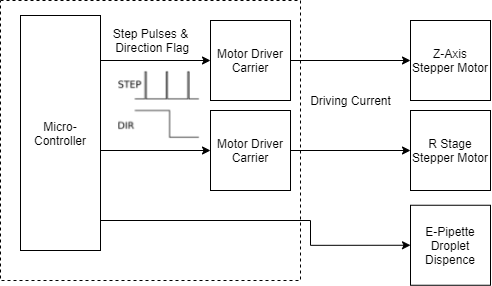
\includegraphics[width=0.4\textwidth]{img/ED_block_diag.png}
    \caption{Block Diagram of Base Electronic Design}
    \label{fig:e_block}
\end{figure}

\subsection{Motor}
The motion required for the motors in this system is to provide rotation about the vertical axis to the mounted pipette, to swing from above the substrate to out of the camera view and over a refill reservoir, as well as continuous rotation to interface the Z axis control for droplet depositing and possible refilling.  

Stepper motors allow for both precise position control without the need for a feedback system and are capable of continuous rotation. In comparison, brushed/brushless DC motors require encoders for positional control and servos may do either but not both continuous rotation and positioning.

NEMA17 standard sized steppers were chosen to best fit the dimensions of the XYZ optical stage (60mm plate to 40mm motor frame) with room for fastening hardware. That left two choices for the top R stage motor; full size 38mm high frame or shorter pancake frame. Even through the pancake frame would reduce the overall height of the system, the shaft length available for this motor is less only 7mm and would greatly restrict the mounting options of the tower to the motor. For this reason 2 NEMA17x38mm Stepper motors were chosen. 

\newpage
\subsection{Motor Drivers}

\subsubsection*{The Requirements}
To drive the selected stepper motors, I decided on discrete step/direction style micro stepping drivers. This allows for the design to be flexible with its electronics placed to accommodate the experimental needs. Allows for a fairly agnostic choice for controller to supply the control signals, and standardised pinouts allow for requirement flexibility and replacements.

\begin{table}[h]
    \centering
    \begin{tabular}{|l|l|l|l|l|}
    \hline
    \textbf{}     & \textbf{A4988} & \textbf{DRV8825} & \textbf{STPIN820} & \textbf{DRV8834} \\ \hline
    Step Res      & 1/16           & 1/32             & 1/256             & 1/32             \\ \hline
    Logic Level   & 3V3/5V         & 3V3/5V           & 3V3/5V            & 3V3/5V           \\ \hline
    Current Limit & 1A             & 1.5A             & 0.9A              & 1.5A             \\ \hline
    Drive Voltage & 8-35V          & 8.2-45V          & 7-48V             & 2.5-10.8         \\ \hline
    \end{tabular}
    \caption{Comparison of considered drivers}
    \end{table}

Main consideration for device choice are: micro step resolution, driving current limit (passively cooled), and configuration pinout.

\subsubsection*{The Choice}
The DRV8825 was ultimately chosen. 
\begin{itemize}
    \item High microstepping resolution, lower than the STPIN820 but cheap high resolution driver are prone to step skipping \cite{step_book}
    \item Highest driving current as torque requirements are unknown for this design the headroom is nice even if it isn't use, especially as it will run cooler at lower power draw. 
    \item It ranked above the DRV8834 due to it configuration pins (to set microstepping mode) as it provide all 3 pins without the requirement to leave pins floating as a setting thus allowing for full software control.
\end{itemize}

\subsection{Auxiliary Components}
In addition to the above primary components lever-action limit switches were also selected if it were to be deemed necessary for the motor controller to have that kind of positional feedback for homing and the like. Shaft mounting hardware was also purchased.

\newpage
\section{Initial Driving Firmware Implementation}
\subsection{Setup and Requirements}
With the parts selected and ordered, I wrote test firmware on an ESP32 to validate its ability in producing the required pulse train step signal. The controller was required to produce N steps (pulses) at a set average speed, and ramp up and down that pulse speed at the head and tail of that signal.

Set values of 200 steps forward and back, at a speed of 200 steps per second, with max acceleration or 800 steps per second per second:

These pulses were captured on a second microcontroller listening for falling edges to trigger an interrupt routine to record and display that data.

\subsection{Results}

Figure \ref{fig:code}:a shows a successfully produced signal of 200 pulses with an inferred acceleration at its head/tail. This speed ramping is better illustrated in figure \ref{fig:code}:b showing the stepping change in pulses per second over the course of the pulse train.

\begin{figure}[h]
    \centering
    \begin{subfigure}{.45\textwidth}
      \centering
      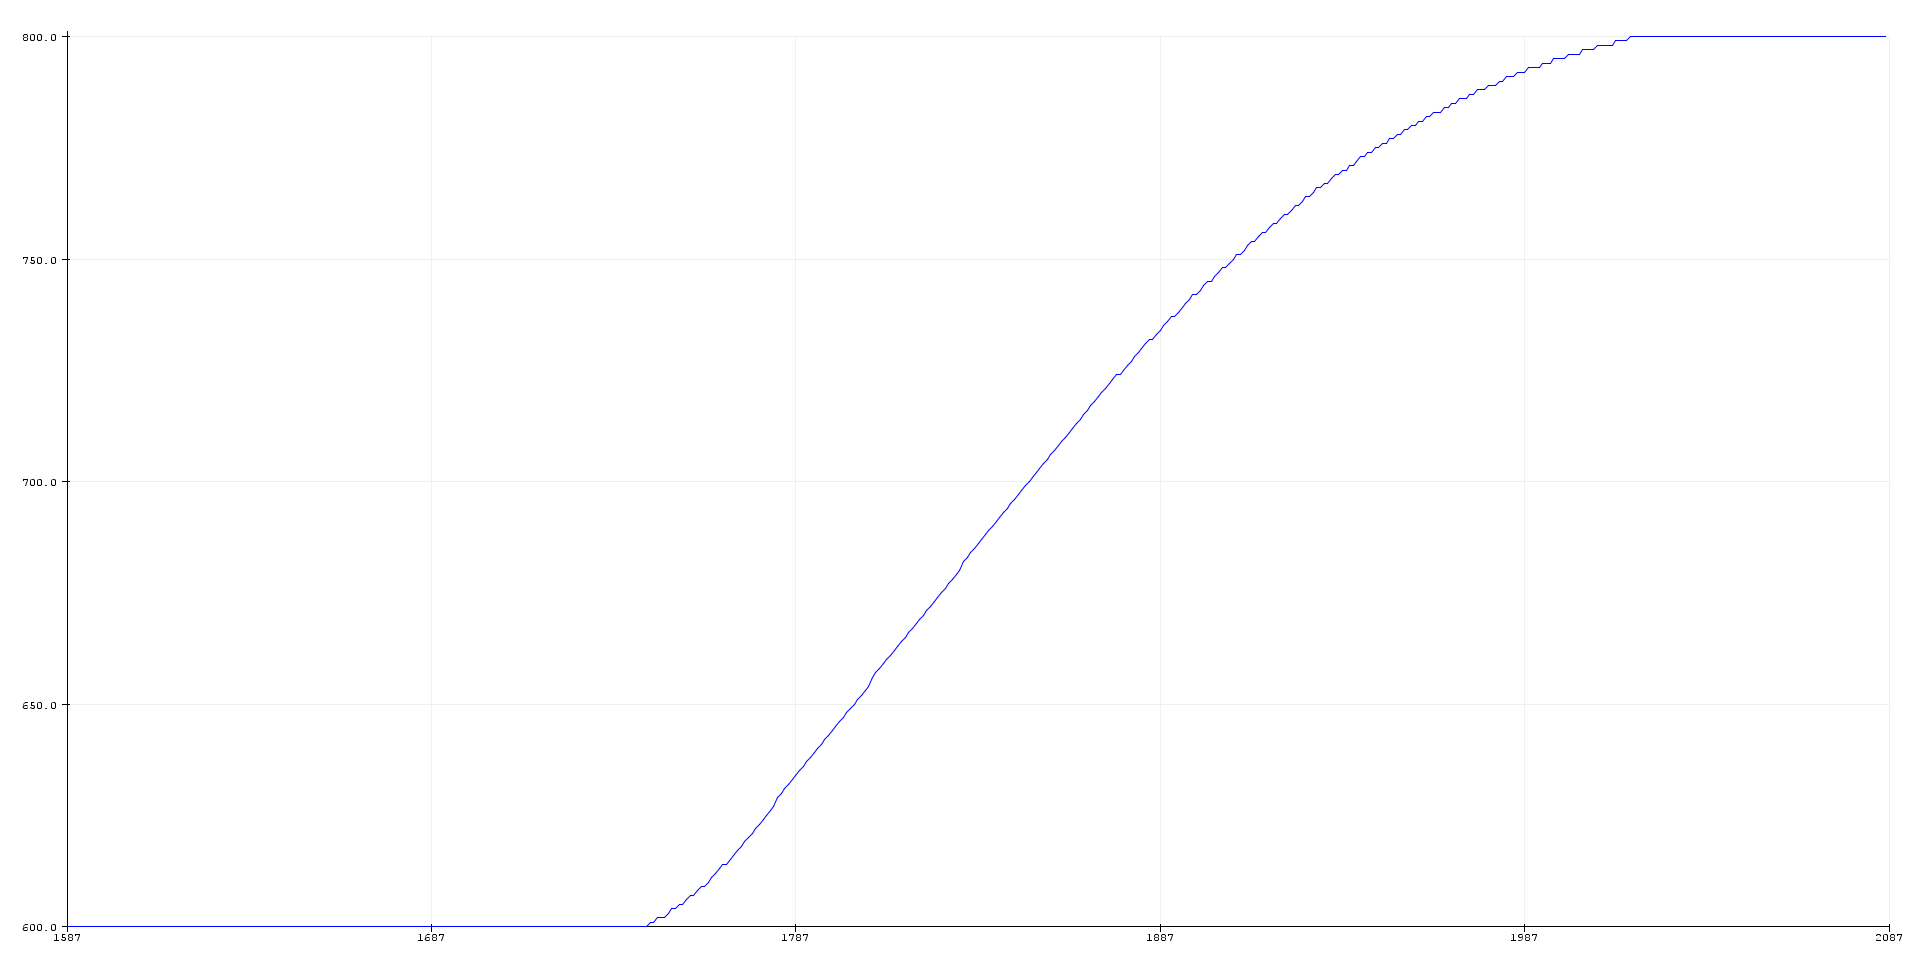
\includegraphics[width=0.8\linewidth]{img/stepper_pulses.PNG}
      \caption{Pulse Count}
    \end{subfigure}%
    \begin{subfigure}{.45\textwidth}
      \centering
      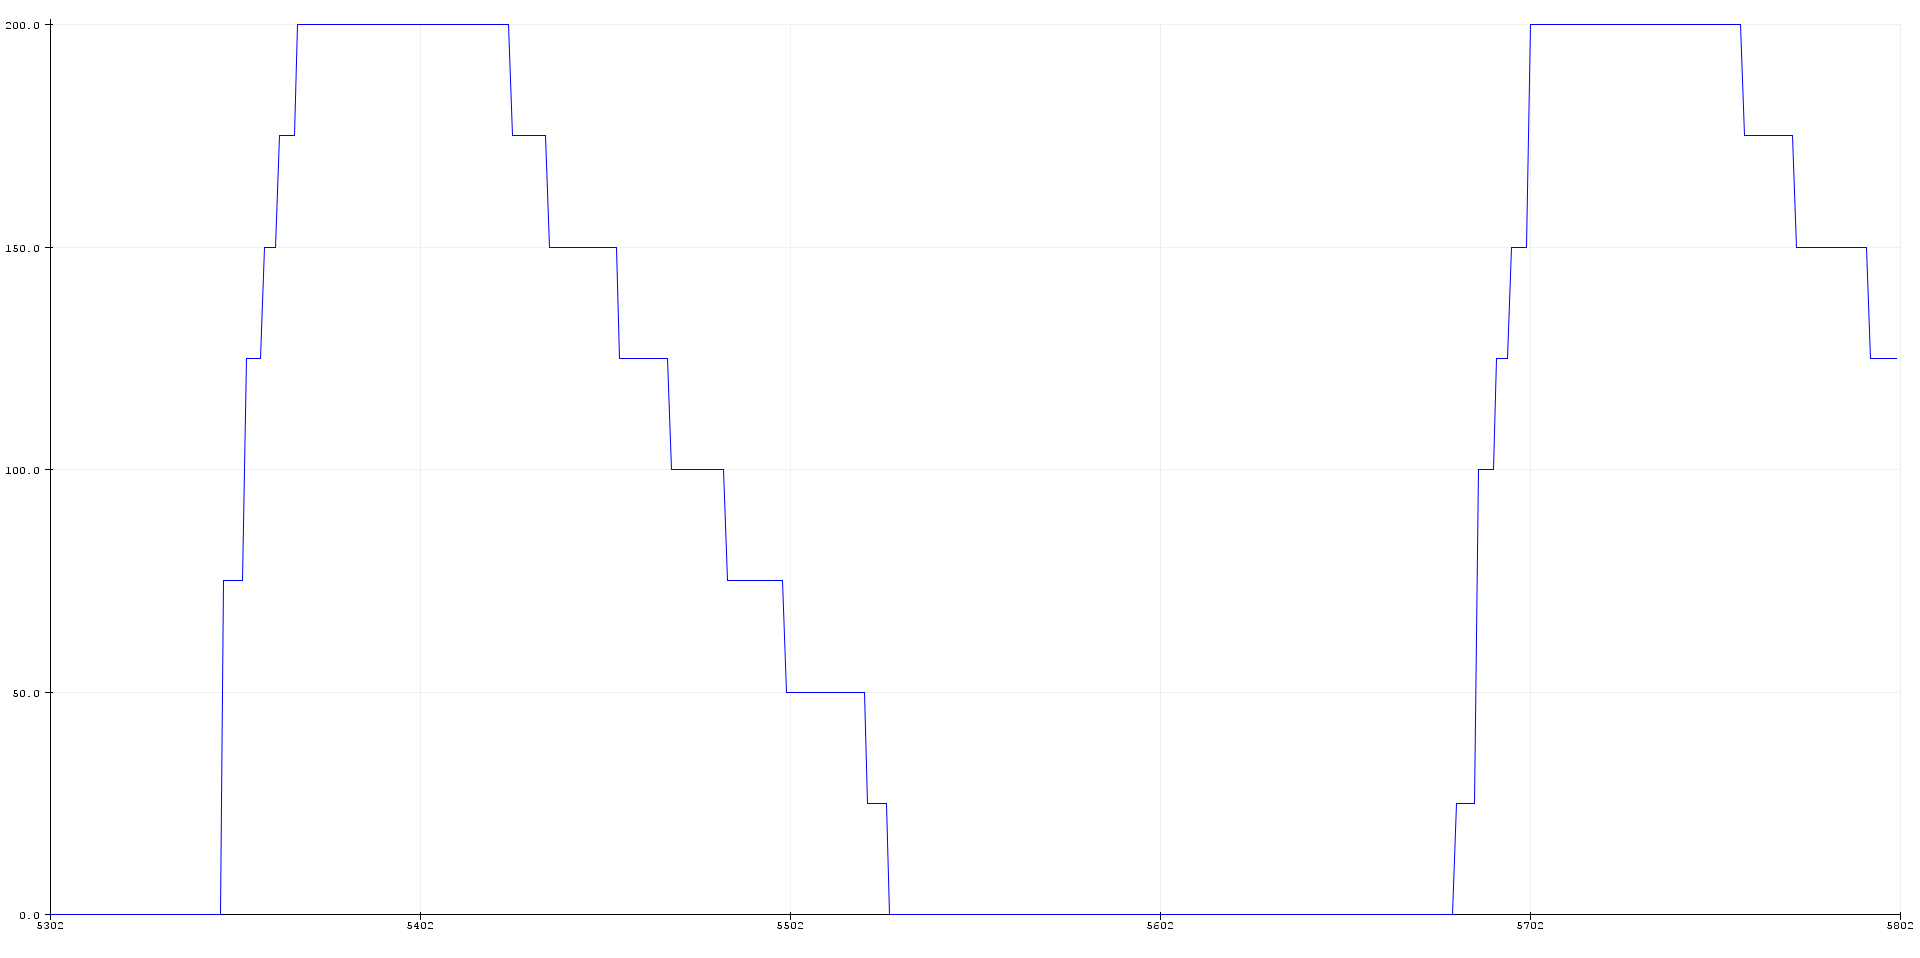
\includegraphics[width=0.8\linewidth]{img/stepper_pulse_acc.PNG}
      \caption{Pulses per Second}
    \end{subfigure}
    \caption{}
    \label{fig:code}
  \end{figure}

  Upon the arrival of the motors themselves it will be determined what the exact requirements for this signal will be to prevent coil stalling and reduce vibrations in the system. It does however leave me with 3 main variables to tune this performance:
  \begin{itemize}
      \item Constant Step Count: What level of micro stepping can be achieved/whether it is required 
      \item Step speed: Limits, usable speeds, stability
      \item Step Acceleration: Motor performance, stall avoidance, resonances
  \end{itemize} 
